\documentclass[12pt,a4paper,titlepage]{article}
\usepackage[utf8]{inputenc}
\usepackage{polski}
\usepackage{listings}
\usepackage{graphicx}
\usepackage{xcolor}
\usepackage{minted}
\usepackage{amsmath}
\usepackage{caption}
 
\DeclareCaptionType{myequation}[][Równanie parametryczne]
\captionsetup[myequation]{labelformat=empty}

\makeatletter
\newcommand{\linia}{\rule{\linewidth}{0.4mm}}
\renewcommand{\maketitle}{\begin{titlepage}
    \vspace*{1cm}
    \begin{center}\small
    Politechnika Wrocławska\\
    Wydział Elektroniki\\
    Grafika Komputerowa i Komunikacja Człowiek-Komputer
    \end{center}
    \vspace{3cm}
    \noindent\linia
    \begin{center}
      \LARGE \textsc{\@title}
         \end{center}
     \linia
    \vspace{0.5cm}
    \begin{flushright}
    \begin{minipage}{7cm}
    \textit{\small Autor:}\\
    \normalsize \textsc{\@author} \par
    \end{minipage}
    \vspace{5cm}

     {\small czwartek, 17\textsuperscript{15}-20\textsuperscript{15} TN}\\
        mgr inż. Szymon Datko
     \end{flushright}
    \vspace*{\stretch{6}}
    \begin{center}
    \@date
    \end{center}
  \end{titlepage}%
}
\makeatother
\author{Justyna Skalska, 225942}
\title{Sprawozdanie nr 2\\
(OpenGL - modelowanie obiektów 3D)}

\begin{document}

\maketitle
\section{Omówienie tematu}
Naszym zadaniem na laboratoriach było stworzenie prostego programu wprowadzającego do modelowania oraz wizualizacji scen 3D z wykorzystaniem biblioteki OpenGL wraz z rozszerzeniem GLUT. Głównym zadaniem było wykonanie modelu jajka przy wykorzystaniu podanych równań parametrycznych. Program miał mieć trzy tryby wyświetlania jajka: z punktów, linii lub kolorowych trójkątów. Obiekt powinien się także obracać podczas wykonywania programu.

\begin{myequation}[H]
\begin{equation}
    \begin{split}
    &x(u,v) = (-90v^5 + 225u^4 -270u^3 + 180u^2 - 45u)cos(\pi v) \\
    &y(u,v) = 160u^4 - 320u^3 + 160u^2 \\
    &z(u,v) = (-90v^5 + 225u^4 -270u^3 + 180u^2 - 45u)sin(\pi v) \\
    &0 \le u \le 1, \; 0 \le v \le 1
    \end{split}
\end{equation}
\caption{Równanie parametryczne jajka}
\end{myequation}

\section{Omówienie kodu}

\begin{listing}[H]
\caption{Zmienne globalne programu}
\begin{minted}[linenos,breaklines]{C++}
struct Point {   // punkt wykorzystywany przez program
  float x, y, z;
};
static GLfloat theta[] = { 0.0, 0.0, 0.0 }; // trzy kąty obrotu
static int N = 20;  // liczba przedziałów
static Point** colors;  // tablica kolorów punktów
int model = 1;  // tryb rysowania w momencie startu programu
\end{minted}
\end{listing}

\begin{listing}[H]
\caption{Funkcja zwracająca losową liczbę}
\begin{minted}[linenos,breaklines]{C++}
float getRand() {
    return float(rand() % 1000) / 1000;
}
\end{minted}
\end{listing}

\begin{listing}[H]
\caption{Funkcja wyliczająca współrzędne krzywej Béziera}
\begin{minted}[linenos,breaklines]{C++}
Point getBezierCurve(float u, float v) {
  float x, y, z;
  x = (-90 * pow(u, 5) + 225 * pow(u, 4) - 270 * pow(u, 3) + 180 *
    pow(u, 2) - 45 * u) * cos(M_PI * v);
  y = 160 * pow(u, 4) - 320 * pow(u, 3) + 160 * pow(u, 2);
  z = (-90 * pow(u, 5) + 225 * pow(u, 4) - 270 * pow(u, 3) + 180 *
    pow(u, 2) - 45 * u) * sin(M_PI * v);

  return { x, y, z }; // koordynaty punktu
}
\end{minted}
\end{listing}

\begin{listing}[H]
\caption{Funkcja zwracająca dwuwymiarową tablicę punktów krzywej Béziera}
\begin{minted}[linenos,breaklines]{C++}
Point** getBezierValues(int n) {
  // pusta dwuwymiarowa tablica na punkty
  Point** bezierValues = new Point*[n + 1];
  for (size_t i = 0; i < n + 1; i++) {
    bezierValues[i] = new Point[n + 1];
  }
  
  // generowanie punktów krzywej według zmiennych u i v
  for (size_t i = 0; i <= n; i++) {
    for (size_t j = 0; j <= n; j++) {
      float u = ((float)i) / n;
      float v = ((float)j) / n;

      bezierValues[i][j] = getBezierCurve(u, v);
    }
  }

  return bezierValues;
}
\end{minted}
\end{listing}

Przy pisaniu tej funkcji napotkałam problem z typem float. W pierwszym podejściu użyłam zmiennej typu float i przypisałam jej wartość: \\ \mintinline{C++}{float interval = 1/n;}. Niestety moje jajko nie wyglądało poprawnie. Okazało się, że "1" musiałam zastąpić przez "1.0f". Przez to drobne niedopatrzenie dane generowane w dalszej części funkcji były złe i jajko nie domykało się odpowiednio. Dopiero zmiana na jedynki na tym float naprawiła problem.\\
Następnie dzięki sugestii prowadzącego zmieniłam sposób generowania wartości zmiennych u i v, dzięki czemu kod stał się czytelniejszy.

\begin{listing}[H]
\caption{Funkcja zwracająca dwuwymiarową tablicę kolorów}
\begin{minted}[linenos,breaklines]{C++}
Point** getColors(int n) {
  // pusta dwuwymiarowa tablica na kolory
  Point** colors = new Point*[n + 1];
  for (size_t i = 0; i < n + 1; i++) {
    colors[i] = new Point[n + 1];
  }

  // przypisanie każdemu puntowi w tablicy losowego koloru
  for (size_t i = 0; i <= n; i++) {
    for (size_t j = 0; j <= n; j++) {
      colors[i][j] = {getRandom(), getRandom(), getRandom()};
    }
  }

  // przypisanie takich samych kolorów punktom leżącym po dwóch stronach złączenia jajka
  for (size_t i = 0; i < n/2; i++) {
    colors[i][n] = colors[n - i][0];
    colors[i][0] = colors[n - i][n];
  }

  return colors;
}
\end{minted}
\end{listing}

\begin{listing}[H]
\caption{Funkcja rysująca jajko złożone z punktów}
\begin{minted}[linenos,breaklines]{C++}
void drawEggFromPoints(int n, Point** bezierValues)
{
  glBegin(GL_POINTS);

  for (size_t i = 0; i <= n; i++) {
    for (size_t j = 0; j <= n; j++) {
      glVertex3f(bezierValues[i][j].x, bezierValues[i][j].y - 5,
        bezierValues[i][j].z);
    }
  }

  glEnd();
}
\end{minted}
\end{listing}

\begin{listing}[H]
\caption{Funkcja rysująca jajko złożone z linii}
\begin{minted}[linenos,breaklines]{C++}
void drawEggFromLines(int n, Point** bezierValues) {
  glBegin(GL_LINES);

  for (size_t i = 0; i < n; i++) {
    for (size_t j = 0; j < n; j++) {
      glVertex3f(bezierValues[i][j].x, bezierValues[i][j].y - 5, 
        bezierValues[i][j].z);
      glVertex3f(bezierValues[i + 1][j].x, bezierValues[i + 1][j].y - 5, 
        bezierValues[i + 1][j].z);
      glVertex3f(bezierValues[i][j].x, bezierValues[i][j].y - 5, 
        bezierValues[i][j].z);
      glVertex3f(bezierValues[i][j + 1].x, bezierValues[i][j + 1].y - 5, 
        bezierValues[i][j + 1].z);
      glVertex3f(bezierValues[i][j].x, bezierValues[i][j].y - 5, 
        bezierValues[i][j].z);
      glVertex3f(bezierValues[i + 1][j + 1].x,
        bezierValues[i + 1][j + 1].y - 5, bezierValues[i + 1][j + 1].z);
    }
  }

  glEnd();
}
\end{minted}
\end{listing}

\begin{listing}[H]
\caption{Funkcja rysująca jajko z trójkątów wraz z losowymi kolorami}
\begin{minted}[linenos,breaklines]{C++}
void drawEggFromTriangles(int n, Point** bezierValues, Point** colors) {
  glBegin(GL_TRIANGLES);
  // każdemu punktowi krzywej przypisany jest kolor z tablicy kolorów
  for (size_t i = 0; i < n; i++) {
    for (size_t j = 0; j < n; j++) {
      glColor3f(colors[i][j].x, colors[i][j].y, colors[i][j].z);
      glVertex3f(bezierValues[i][j].x, bezierValues[i][j].y - 5, 
        bezierValues[i][j].z);
      glColor3f(colors[i + 1][j].x, colors[i + 1][j].y,
        colors[i + 1][j].z);
      glVertex3f(bezierValues[i + 1][j].x, bezierValues[i + 1][j].y - 5, 
        bezierValues[i + 1][j].z);
      glColor3f(colors[i + 1][j + 1].x, colors[i + 1][j + 1].y,
        colors[i + 1][j + 1].z);
      glVertex3f(bezierValues[i + 1][j + 1].x,
        bezierValues[i + 1][j + 1].y - 5, bezierValues[i + 1][j + 1].z);

      glColor3f(colors[i][j + 1].x, colors[i][j + 1].y,
        colors[i][j + 1].z);
      glVertex3f(bezierValues[i][j + 1].x, bezierValues[i][j + 1].y - 5, 
        bezierValues[i][j + 1].z);
      glColor3f(colors[i][j].x, colors[i][j].y, colors[i][j].z);
      glVertex3f(bezierValues[i][j].x, bezierValues[i][j].y - 5, 
        bezierValues[i][j].z);
      glColor3f(colors[i + 1][j + 1].x, colors[i + 1][j + 1].y,
        colors[i + 1][j + 1].z);
      glVertex3f(bezierValues[i + 1][j + 1].x,
        bezierValues[i + 1][j + 1].y - 5, bezierValues[i + 1][j + 1].z);
    }
  }

  glEnd();
}
\end{minted}
\end{listing}

\begin{listing}[H]
\caption{Funkcja rysująca jajko w trybie wybranym przez użytkownika}
\begin{minted}[linenos,breaklines]{C++}
void drawEgg(int n) {
  // dwuwymiarowa tablica współrzędnych krzywej Béziera
  Point** bezierValues = getBezierValues(n);

  // obracanie jajka
  glRotatef(theta[0], 1.0, 0.0, 0.0);
  glRotatef(theta[1], 0.0, 1.0, 0.0);
  glRotatef(theta[2], 0.0, 0.0, 1.0);

  if (model == 1) {
    drawEggFromPoints(n, bezierValues);
  }
  else if (model == 2) {
    drawEggFromLines(n, bezierValues);
  } else {
    drawEggFromTriangles(n, bezierValues, colors);
  }
}
\end{minted}
\end{listing}
\newpage
\section{Rezultat prac}
Udało mi się wykonać wszystkie podpunkty zadania. Dzięki wykonanemu ćwiczeniu mogłam zapoznać się z podstawami modelowania i wizualizacji 3D. Podczas wykonywania zadania miałam problem z generowaniem kolorów jajka tak, aby niewidoczne było miejsce łączenia jajka. Rozwiązałam to pętlą, która przypisuje odpowiednie kolory punktom na złączeniach. Wiedza jak rozwiązywać takie problemy może przydać się przy pisaniu następnych programów rysujących modele 3D.

\begin{figure}[H]
\centering
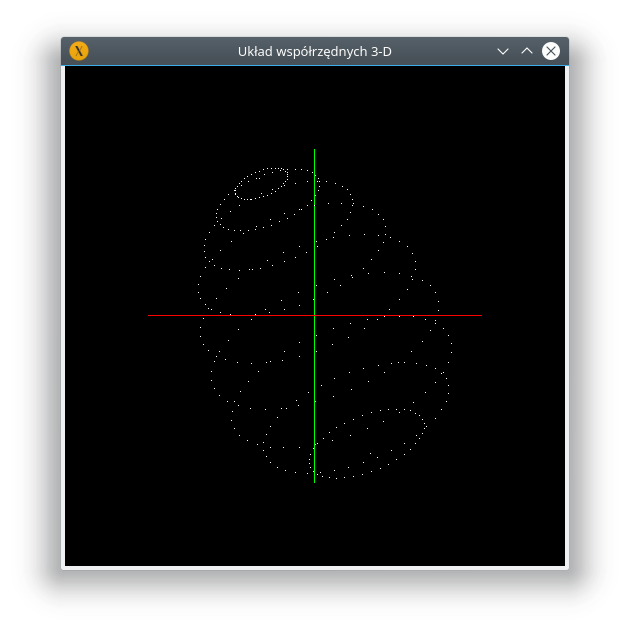
\includegraphics[width = 9cm]{images/egg_points.png}
\caption{Jajko złożone z punktów}
\label{fig:eggPoints}
\end{figure}

\begin{figure}[H]
\centering
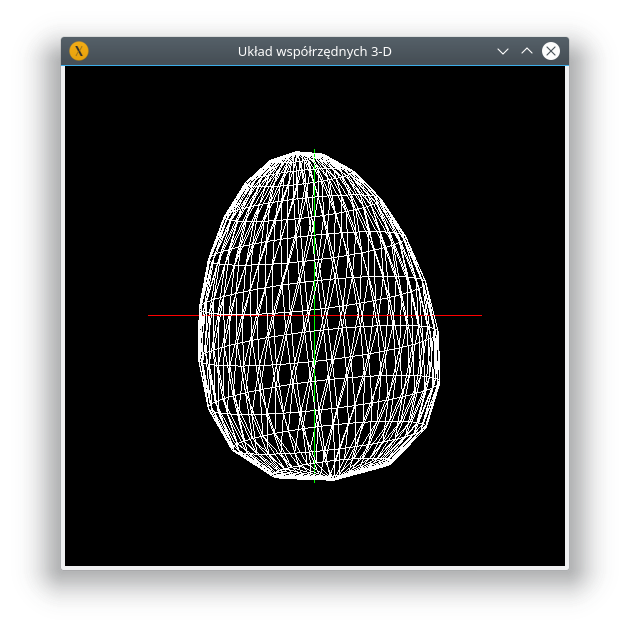
\includegraphics[width = 9cm]{images/egg_lines.png}
\caption{Jajko złożone z linii}
\label{fig:eggLines}
\end{figure}

\begin{figure}[H]
\centering
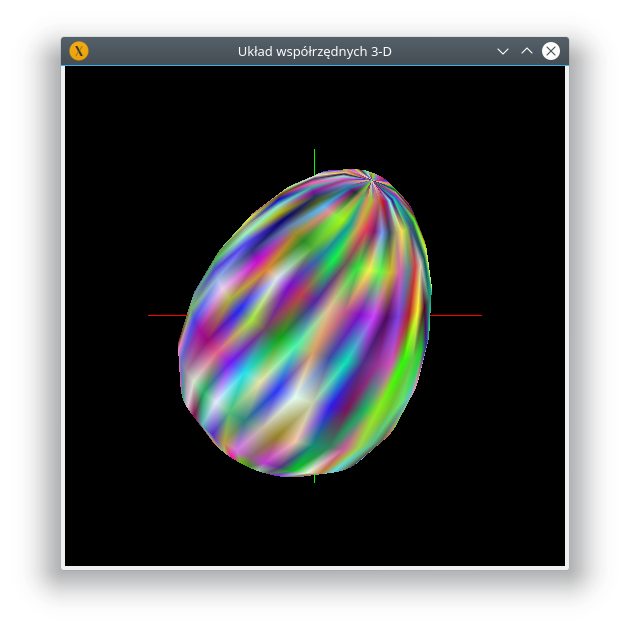
\includegraphics[width = 9cm]{images/egg_triangles.png}
\caption{Jajko złożone z trójkątów}
\label{fig:eggTriangles}
\end{figure}

\end{document}
